% Created 2019-01-10 Thu 13:51
% Intended LaTeX compiler: pdflatex
\documentclass[11pt]{article}
\usepackage[utf8]{inputenc}
\usepackage[T1]{fontenc}
\usepackage{graphicx}
\usepackage{grffile}
\usepackage{longtable}
\usepackage{wrapfig}
\usepackage{rotating}
\usepackage[normalem]{ulem}
\usepackage{amsmath}
\usepackage{textcomp}
\usepackage{amssymb}
\usepackage{capt-of}
\usepackage{hyperref}
\usepackage{minted}
\usepackage[hyperref,x11names]{xcolor}
\usepackage{physics}
\usepackage{cases}
\graphicspath{ {./} }
\usepackage{tikz}
\usetikzlibrary{arrows,plotmarks,calc,positioning,fit}
\usetikzlibrary{shapes.geometric, decorations.pathmorphing, patterns, backgrounds}
\newcommand{\tikzremember}[1]{{  \tikz[remember picture,overlay]{\node (#1) at (0,11pt) { };}}}
\tikzset{snake it/.style={decorate, decoration=snake}}
\usepackage[nottoc]{tocbibind}
\author{Tigany Zarrouk}
\date{\today}
\title{things-to-do}
\hypersetup{
 pdfauthor={Tigany Zarrouk},
 pdftitle={things-to-do},
 pdfkeywords={},
 pdfsubject={},
 pdfcreator={Emacs 25.3.1 (Org mode 9.1.14)}, 
 pdflang={English}}
\begin{document}

\maketitle
\tableofcontents

\section{Unrelaxed 09/01/19}
\label{sec:org43dac11}
From Girshick 
\begin{center}
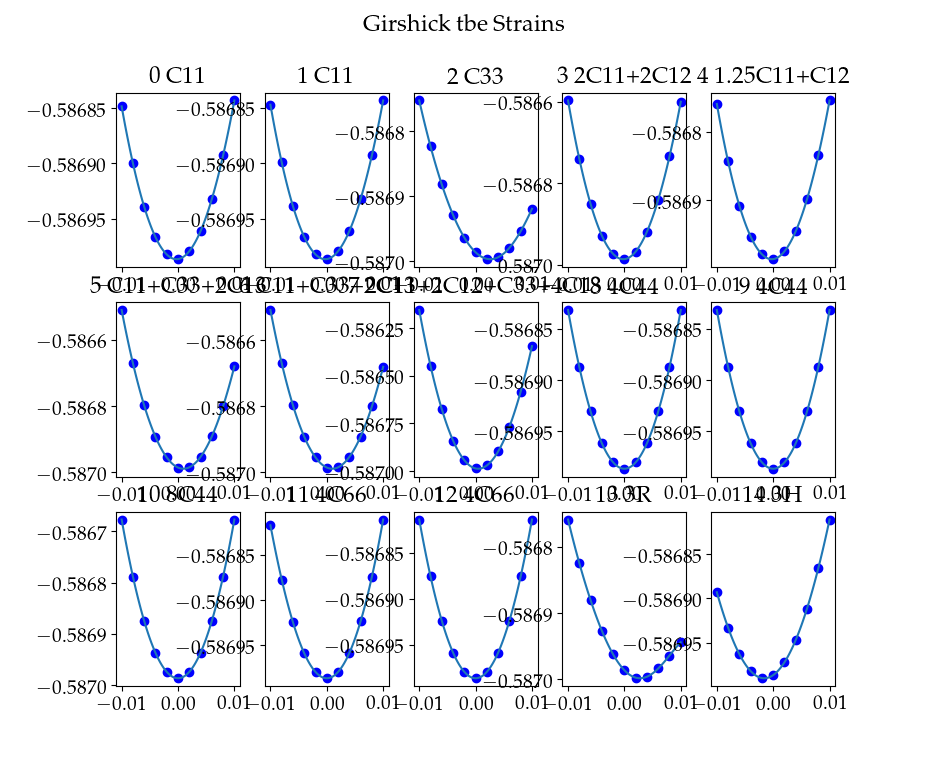
\includegraphics[width=.9\linewidth]{Images/girshick_ec_09-01-19.png}
\end{center}
\begin{minted}[]{python}
C11 =  179.4105487815,   C11_exp =  176.1000000000
C33 =  199.7411232511,   C33_exp =  190.5000000000
C44 =  49.2452549871,   C44_exp =  50.8000000000
C66 =  55.1996755007,   C66_exp =  44.6000000000
C12 = -12062.1968073992,   C12_exp =  86.9000000000
C13 = -11773.0959208918,   C13_exp =  68.3000000000
K =  103.7213715237,   K_FR =  109.9666666667
R =  67.3715578360,   R_FR =  61.8000000000
H =  58.5592139578,   H_FR =  45.9650000000 

\end{minted}

\begin{center}
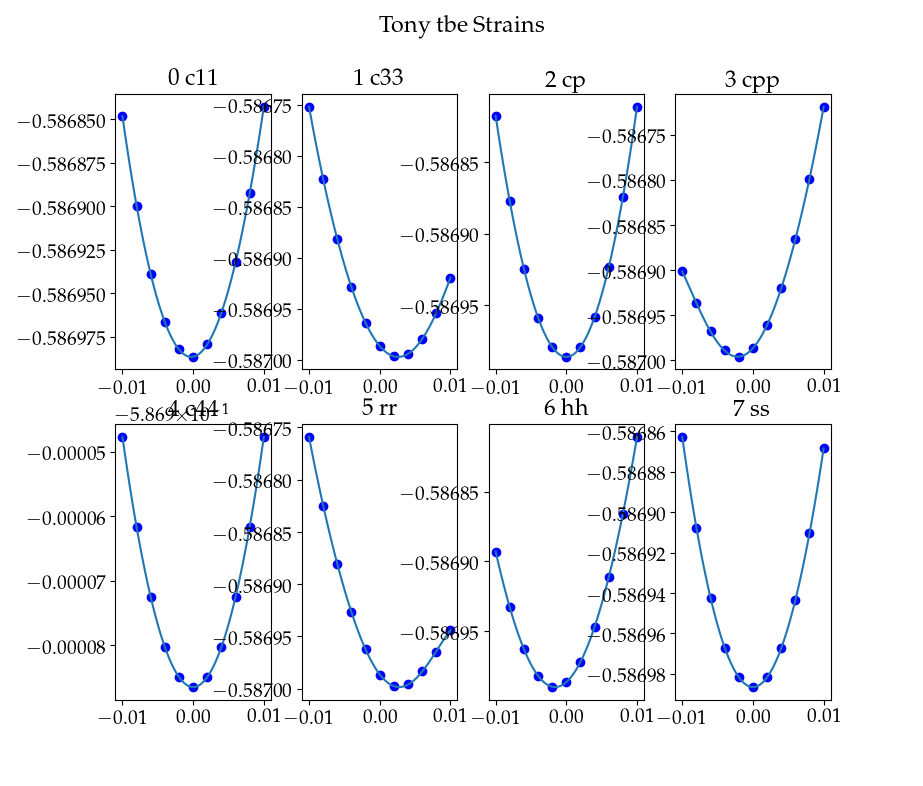
\includegraphics[width=.9\linewidth]{Images/tony_ec_09-01-19.png}
\end{center}
From Tony
\begin{minted}[]{python}
C11 =  179.4144752885,   C11_exp =  176.1000000000
C33 =  199.7411232511,   C33_exp =  190.5000000000
C44 =  49.2723940787,   C44_exp =  50.8000000000
C66 =  220.7854442689,   C66_exp =  44.6000000000
C12 = -262.1564132494,   C12_exp =  86.9000000000
C13 = -324.7738952427,   C13_exp =  68.3000000000
K = -1264.8383336416,   K_FR =  109.9666666667
R =  807.9179447561,   R_FR =  61.8000000000
H =  698.7467357942,   H_FR =  45.9650000000 

\end{minted}
\section{Relaxed 09/01/19}
\label{sec:orge2893fe}
\subsection{gtol = 1e-6}
\label{sec:org42d04e1}
\begin{center}
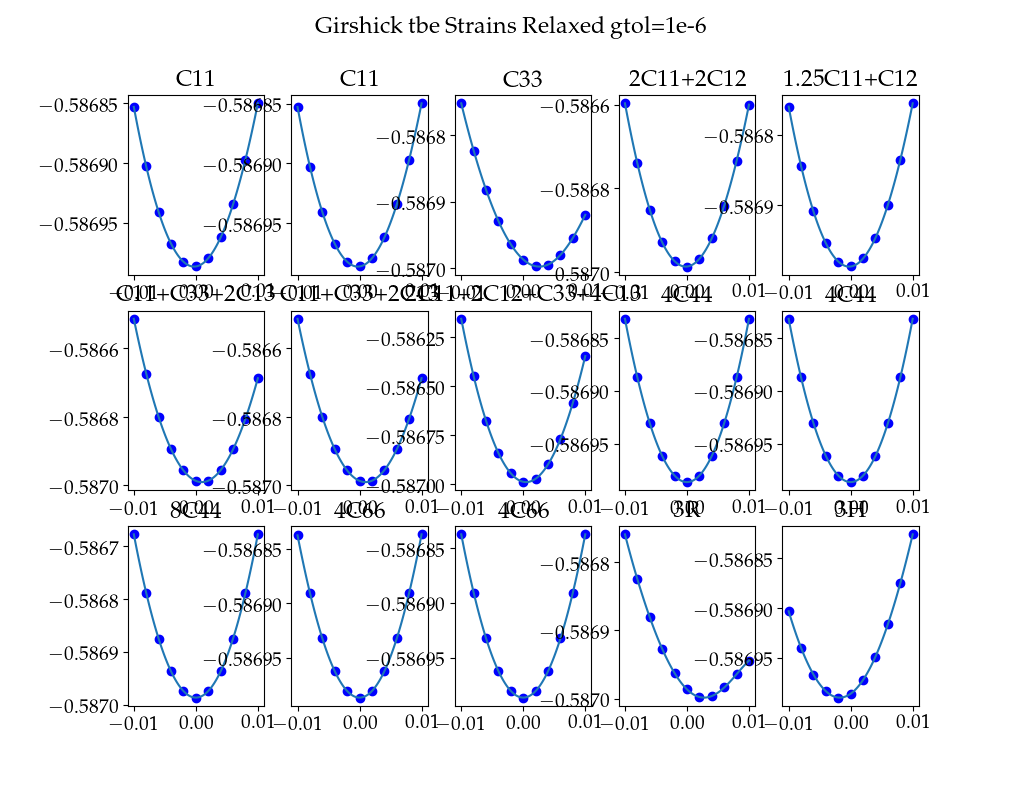
\includegraphics[width=.9\linewidth]{Images/girshick_ec_09-01-19_gtol1e-6.png}
\end{center}
Girshick 
\begin{minted}[]{python}
 C11 =  172.9087030436,   C11_exp =  176.1000000000
 C33 =  198.5744121594,   C33_exp =  190.5000000000
 C44 =  49.2523330247,   C44_exp =  50.8000000000
 C66 =  48.0100583268,   C66_exp =  44.6000000000
 C12 = -11615.4942407936,   C12_exp =  86.9000000000
 C13 = -11535.5170624530,   C13_exp =  68.3000000000
 K =  103.1312742638,   K_FR =  109.9666666667
 R =  65.5404379802,   R_FR =  61.8000000000
 H =  54.3174856150,   H_FR =  45.9650000000 

Girshick CURVATURES GPa 
 [0.0, 172.9004311080267, 172.9169749790961, 198.57441215940486, 497.48462721215066, 292.5218297904287, 486.695326183829, 486.7329294063404, 928.1814683742241, 197.14858238024067, 197.09765185486694, 393.79109416080956, 192.17246592014106, 191.90800069434025, 196.6213139405376, 162.95245684504613] 

Polynomial coeffs 0 
 [ 2.403846172680e+03 -6.920163181274e+01 -6.273310025869e+00  1.357572843835e+00  7.517680653379e-04 -5.869865103730e-01]

Polynomial coeffs 1 
 [ 1.903044861896e+03 -4.334207465834e+01 -6.200648309028e+00  1.357754953393e+00  7.540378787786e-04 -5.869865113054e-01]

Polynomial coeffs 2 
 [-4.917868589163e+04 -6.796328672108e+02  3.263585371778e+00  1.574863053623e+00 -8.199050699247e-03 -5.869864952914e-01]

Polynomial coeffs 3 
 [ 3.205128206180e+04 -3.898965618549e+02 -1.980113636524e+01  3.916451777404e+00  1.496786130586e-03 -5.869865149184e-01]

Polynomial coeffs 4 
 [ 9.465144240806e+03 -1.305725525278e+02 -9.881173515241e+00  2.297486159688e+00  1.126506118904e-03 -5.869865121212e-01]

Polynomial coeffs 5 
 [-5.809294876445e+03 -9.852127061358e+01 -1.135453088524e+01  3.868858537321e+00 -7.467478438242e-03 -5.869865101165e-01]

Polynomial coeffs 6 
 [-6.310096153941e+03 -8.322406783073e+01 -1.124981789038e+01  3.868797348514e+00 -7.467399766901e-03 -5.869865112354e-01]

Polynomial coeffs 7 
 [-4.006410093002e+02  6.337412569028e+01 -2.770032051469e+01  7.360139860159e+00 -6.716937062899e-03 -5.869865079021e-01]

Polynomial coeffs 8 
 [ 6.558740582196e-07 -6.337412596426e+01 -1.619448271167e-10  1.554425990689e+00  7.588095945650e-15 -5.869865174592e-01]

Polynomial coeffs 9 
 [ 1.332430917251e-05 -5.463286706175e+01 -1.964485796358e-09  1.554023892774e+00  5.655976830621e-14 -5.869865153613e-01]

Polynomial coeffs 10 
 [ 6.892467635713e-07 -1.700903263886e+02 -1.655851650898e-10  3.104864510502e+00  7.639041260611e-15 -5.869864947086e-01]

Polynomial coeffs 11 
 [ 1.036658653955e+04 -2.354676574146e+02 -5.373142481023e-01  1.515364947563e+00 -4.065559458558e-06 -5.869865112587e-01]

Polynomial coeffs 12 
 [-7.785735317634e-06 -2.225378791006e+02  1.384014746019e-09  1.513116258773e+00 -5.405862742570e-14 -5.869864990443e-01]

Polynomial coeffs 13 
 [-1.664162660344e+05 -2.467038170221e+03  1.228884396969e+01  1.593577360145e+00 -8.816020687671e-03 -5.869863451515e-01]

Polynomial coeffs 14 
 [ 1.096754809783e+04 -3.547494172056e+02 -7.043360288293e+00  1.255349650346e+00  4.476896561852e-03 -5.869865091142e-01]

\end{minted}


Tony
\begin{center}
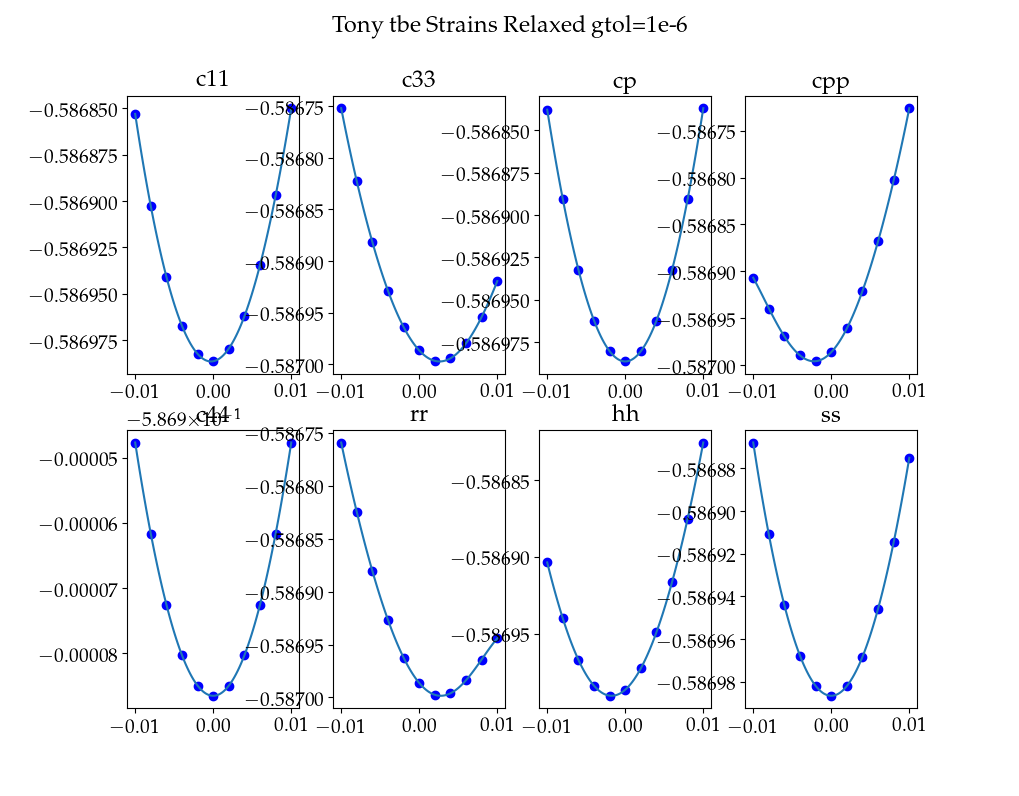
\includegraphics[width=.9\linewidth]{Images/tony_ec_09-01-19_gtol1e-6.png}
\end{center}
\begin{minted}[]{python}
 C11 =  173.0346579154,   C11_exp =  176.1000000000
 C33 =  198.5744121594,   C33_exp =  190.5000000000
 C44 =  49.2568530334,   C44_exp =  50.8000000000
 C66 =  191.9023467596,   C66_exp =  44.6000000000
 C12 = -210.7700356038,   C12_exp =  86.9000000000
 C13 = -317.8089744286,   C13_exp =  68.3000000000
 K = -1148.1322409320,   K_FR =  109.9666666667
 R =  815.3246721725,   R_FR =  61.8000000000
 H =  635.6114482523,   H_FR =  45.9650000000 

Tony CURVATURES GPa 
[0.0, 173.03465791544974, 198.57441215940486, 191.9023467596449, 251.80675473303774, 49.256853033364514, 196.6213139405376, 163.8312829442945, 146.72504872873364]

Polynomial coeffs 0 
 [ 4.507211527019e+03 -8.449883471457e+01 -6.437754951847e+00  1.358490676015e+00  7.541054778124e-04 -5.869865162471e-01]

Polynomial coeffs 1 
 [-4.917868589163e+04 -6.796328672108e+02  3.263585371778e+00  1.574863053623e+00 -8.199050699247e-03 -5.869864952914e-01]

Polynomial coeffs 2 
 [ 8.463541680370e+03 -2.123397437739e+02 -3.994573151874e-01  1.513192016341e+00 -1.159964998503e-06 -5.869865029371e-01]

Polynomial coeffs 3 
 [ 1.832431891172e+05 -2.767883158595e+03 -1.595434513613e+01  1.976062791391e+00  8.808944930130e-03 -5.869863668531e-01]

Polynomial coeffs 4 
 [ 1.810477061546e-05 -2.549533859606e+00 -2.196695165670e-09  3.883668415017e-01  4.328971618917e-14 -5.869865119580e-01]

Polynomial coeffs 5 
 [-1.664162660344e+05 -2.467038170221e+03  1.228884396969e+01  1.593577360145e+00 -8.816020687671e-03 -5.869863451515e-01]

Polynomial coeffs 6 
 [ 2.328725961840e+04 -3.853438230453e+02 -8.112889714681e+00  1.257934149210e+00  4.483477564102e-03 -5.869865099068e-01]

Polynomial coeffs 7 
 [-9.014423067864e+02 -5.754662013020e+01 -3.494500291531e+00  1.155801282067e+00  4.609557103966e-07 -5.869865136131e-01]

\end{minted}
\end{document}
